\documentclass[
	% -- opções da classe memoir --
	12pt,				% tamanho da fonte
	openright,			% capítulos começam em pág ímpar (insere página vazia caso preciso)
	twoside,			% para impressão em recto e verso. Oposto a oneside
	a4paper,			% tamanho do papel. 
	% -- opções da classe abntex2 --
	%chapter=TITLE,		% títulos de capítulos convertidos em letras maiúsculas
	%section=TITLE,		% títulos de seções convertidos em letras maiúsculas
	%subsection=TITLE,	% títulos de subseções convertidos em letras maiúsculas
	%subsubsection=TITLE,% títulos de subsubseções convertidos em letras maiúsculas
	% -- opções do pacote babel --
	english,			% idioma adicional para hifenização
	brazil				% o último idioma é o principal do documento
	]{abntex2}

% Pacotes básicos 
\usepackage{lmodern}			% Usa a fonte Latin Modern			
\usepackage[T1]{fontenc}		% Selecao de codigos de fonte.
\usepackage[utf8]{inputenc}		% Codificacao do documento (conversão automática dos acentos)
\usepackage{indentfirst}		% Indenta o primeiro parágrafo de cada seção.
\usepackage{color}				% Controle das cores
\usepackage{graphicx}			% Inclusão de gráficos
\usepackage{microtype} 			% para melhorias de justificação

% Pacote de glossario
\usepackage{./9_Extras/styles/anbtex2-glossario}

% Pacotes de citações
\usepackage[brazilian,hyperpageref]{backref}	 % Paginas com as citações na bibl
\usepackage[alf,abnt-emphasize=bf]{abntex2cite}	% Citações padrão ABNT
% Usado sem a opção hyperpageref de backref
\renewcommand{\backrefpagesname}{Citado na(s) página(s):~}
% Texto padrão antes do número das páginas
\renewcommand{\backref}{}
% Define os textos da citação
\renewcommand*{\backrefalt}[4]{
	\ifcase #1 %
		Nenhuma citação no texto.%
	\or
		Citado na página #2.%
	\else
		Citado #1 vezes nas páginas #2.%
	\fi}%

% Pacotes para algoritmos
\usepackage{listings}
\renewcommand{\lstlistlistingname}{Lista de códigos-fonte} 
\renewcommand{\lstlistingname}{Código-fonte} 
\newlistof{lstlistoflistings}{lol}{\lstlistlistingname}

% Configuracoes gerais
%\lstset{ 
%  backgroundcolor=\color{white},   % choose the background color; you must add \usepackage{color} or \usepackage{xcolor}; should come as last argument
%  basicstyle=\footnotesize,        % the size of the fonts that are used for the code
%  breakatwhitespace=false,         % sets if automatic breaks should only happen at whitespace
%  breaklines=true,                 % sets automatic line breaking
%  captionpos=b,                    % sets the caption-position to bottom
%  commentstyle=\color{mygreen},    % comment style
%  deletekeywords={...},            % if you want to delete keywords from the given language
%  escapeinside={\%*}{*)},          % if you want to add LaTeX within your code
%  extendedchars=true,              % lets you use non-ASCII characters; for 8-bits encodings only, does not work with UTF-8
%  firstnumber=1000,                % start line enumeration with line 1000
%  frame=single,	                   % adds a frame around the code
%  keepspaces=true,                 % keeps spaces in text, useful for keeping indentation of code (possibly needs columns=flexible)
%  keywordstyle=\color{blue},       % keyword style
%  morekeywords={*,...},            % if you want to add more keywords to the set
%  numbers=left,                    % where to put the line-numbers; possible values are (none, left, right)
%  numbersep=5pt,                   % how far the line-numbers are from the code
%  numberstyle=\tiny\color{mygray}, % the style that is used for the line-numbers
%  rulecolor=\color{black},         % if not set, the frame-color may be changed on line-breaks within not-black text (e.g. comments (green here))
%  showspaces=false,                % show spaces everywhere adding particular underscores; it overrides 'showstringspaces'
%  showstringspaces=false,          % underline spaces within strings only
%  showtabs=false,                  % show tabs within strings adding particular underscores
%  stepnumber=2,                    % the step between two line-numbers. If it's 1, each line will be numbered
%  stringstyle=\color{mymauve},     % string literal style
%  tabsize=2,	                   % sets default tabsize to 2 spaces
%  title=\lstname                   % show the filename of files included with \lstinputlisting; also try caption instead of title
%}

\definecolor{listings_keyword}{RGB}{30,80,179}
\definecolor{listings_comment}{RGB}{82,151,82}
\definecolor{listings_identifier}{RGB}{0,0,0}
\definecolor{listings_string}{RGB}{225,89,89}
\definecolor{listings_emphs}{RGB}{159,77,153}
\lstset{
  belowcaptionskip=1\baselineskip,
  breaklines=true,
  frame=tbL,
  showstringspaces=false,
  basicstyle=\footnotesize\ttfamily,
  keywordstyle=\bfseries\color{listings_keyword},
  commentstyle=\itshape\color{listings_comment},
  identifierstyle=\color{listings_identifier},
  emphstyle=\color{listings_emphs},
  stringstyle=\color{listings_string},
  captionpos=b,
  escapechar=\§,
}

% Ajustes para linguagem Python
\lstdefinestyle{Python_lang}{
  language=Python,
  morekeywords={as},
  emph={import,return},
}


\usepackage{amsmath, amssymb}
% \usepackage{pgf}

% CONFIGURAÇÕES DE PACOTES

% Informações de dados para CAPA e FOLHA DE ROSTO
\titulo{Controle de planta didática utilizando Controle Preditivo Baseado em Modelo (MPC)}
\autor{Tiago Correa Prata}
\local{São Paulo}
\data{2019}
\orientador{Alexandre Brincalepe Campo}
%\coorientador{----}
\instituicao{Instituto Federal de São Paulo - IFSP}
\tipotrabalho{Tese (Mestrado)}
% O preambulo deve conter o tipo do trabalho, o objetivo, 
% o nome da instituição e a área de concentração 
\preambulo{Projeto de pesquisa apresentado ao Instituto Federal de Educação, Ciência
e Tecnologia de São Paulo para a qualificação no programa de mestrado em engenharia
de automação e controle.}


% informações do PDF
\definecolor{PDF_blue}{RGB}{28,3,126}
\makeatletter
\hypersetup{
     	%pagebackref=true,
		pdftitle={\@title}, 
		pdfauthor={\@author},
    	pdfsubject={\imprimirpreambulo},
	    pdfcreator={LaTeX},
		pdfkeywords={MPC}{Model Predictive Control}{Controle Avançado}, 
		colorlinks=true,       		% false: boxed links; true: colored links
    	linkcolor=PDF_blue,          	% color of internal links
    	citecolor=PDF_blue,        		% color of links to bibliography
    	filecolor=magenta,      		% color of file links
		urlcolor=PDF_blue,
		bookmarksdepth=4
}
\makeatother

\usepackage[nameinlink, brazilian]{cleveref}

% Posiciona figuras e tabelas no topo da página quando adicionadas sozinhas
% em um página em branco.
\makeatletter
\setlength{\@fptop}{5pt} % Set distance from top of page to first float
\makeatother

% Possibilita criação de Quadros e Lista de quadros.
\newcommand{\quadroname}{Quadro}
\newcommand{\listofquadrosname}{Lista de quadros}

\newfloat[chapter]{quadro}{loq}{\quadroname}
\newlistof{listofquadros}{loq}{\listofquadrosname}
\newlistentry{quadro}{loq}{0}

% configurações para atender às regras da ABNT
\setfloatadjustment{quadro}{\centering}
\counterwithout{quadro}{chapter}
\renewcommand{\cftquadroname}{\quadroname\space} 
\renewcommand*{\cftquadroaftersnum}{\hfill--\hfill}

\setfloatlocations{quadro}{hbtp}

% Espaçamentos entre linhas e parágrafos 

% O tamanho do parágrafo é dado por:
\setlength{\parindent}{1.3cm}

% Controle do espaçamento entre um parágrafo e outro:
\setlength{\parskip}{0.2cm}  % tente também \onelineskip

% compila o indice
\makeindex

% GLOSSARIO
\makeglossaries

%% ---
%% entradas do glossario
%% ---
% \newglossaryentry{pai}{
%                name={pai},
%                plural={pai},
%                description={este é uma entrada pai, que possui outras
%                subentradas.} }
%
% \newglossaryentry{componente}{
%                name={componente},
%                plural={componentes},
%                parent=pai,
%                description={descriação da entrada componente.} }
% 
% \newglossaryentry{filho}{
%                name={filho},
%                plural={filhos},
%                parent=pai,
%                description={isto é uma entrada filha da entrada de nome
%                \gls{pai}. Trata-se de uma entrada irmã da entrada
%                \gls{componente}.} }
% 
%\newglossaryentry{equilibrio}{
%                name={equilíbrio da configuração},
%                see=[veja também]{componente},
%                description={consistência entre os \glspl{componente}}
%                }
%
%\newglossaryentry{latex}{
%                name={LaTeX},
%                description={ferramenta de computador para autoria de
%                documentos criada por D. E. Knuth} }
%
%\newglossaryentry{abntex2}{
%                name={abnTeX2},
%                see=latex,
%                description={suíte para LaTeX que atende os requisitos das
%                normas da ABNT para elaboração de documentos técnicos e científicos brasileiros} }
%% ---

% Exemplo de configurações do glossairo
\renewcommand*{\glsseeformat}[3][\seename]{\textit{#1}  
\glsseelist{#2}}

% ----------------------------------------------------------
% Início do documento
\begin{document}

% Seleciona o idioma do documento (conforme pacotes do babel)
%\selectlanguage{english}
\selectlanguage{brazil}

% Retira espaço extra obsoleto entre as frases.
\frenchspacing 

% ELEMENTOS PRÉ-TEXTUAIS
% \pretextual

% Capa
\imprimircapa

% Folha de rosto
% (o * indica que haverá a ficha bibliográfica)
\imprimirfolhaderosto
% \imprimirfolhaderosto*	% TODO: Substituir por essa linha quando inserir Ficha Catalografica

% Inserir a ficha bibliografica
%% Isto é um exemplo de Ficha Catalográfica, ou ``Dados internacionais de
% catalogação-na-publicação''. Você pode utilizar este modelo como referência. 
% Porém, provavelmente a biblioteca da sua universidade lhe fornecerá um PDF
% com a ficha catalográfica definitiva após a defesa do trabalho. Quando estiver
% com o documento, salve-o como PDF no diretório do seu projeto e substitua todo
% o conteúdo de implementação deste arquivo pelo comando abaixo:
%
% \begin{fichacatalografica}
%     \includepdf{fig_ficha_catalografica.pdf}
% \end{fichacatalografica}

\begin{fichacatalografica}
	\sffamily
	\vspace*{\fill}					% Posição vertical
	\begin{center}					% Minipage Centralizado
	\fbox{\begin{minipage}[c][8cm]{13.5cm}		% Largura
	\small
	\imprimirautor
	%Sobrenome, Nome do autor
	
	\hspace{0.5cm} \imprimirtitulo  / \imprimirautor. --
	\imprimirlocal, \imprimirdata-
	
	\hspace{0.5cm} \thelastpage p. : il. (algumas color.) ; 30 cm.\\
	
	\hspace{0.5cm} \imprimirorientadorRotulo~\imprimirorientador\\
	
	\hspace{0.5cm}
	\parbox[t]{\textwidth}{\imprimirtipotrabalho~--~\imprimirinstituicao,
	\imprimirdata.}\\
	
	\hspace{0.5cm}
		1. Palavra-chave1.
		2. Palavra-chave2.
		2. Palavra-chave3.
		I. Orientador.
		II. Instituto Federal de São Paulo.
		III. Título 			
	\end{minipage}}
	\end{center}
\end{fichacatalografica}

% Inserir errata
%\include{./1_pretext/errata}

% Inserir folha de aprovação
% Isto é um exemplo de Folha de aprovação, elemento obrigatório da NBR
% 14724/2011 (seção 4.2.1.3). Você pode utilizar este modelo até a aprovação
% do trabalho. Após isso, substitua todo o conteúdo deste arquivo por uma
% imagem da página assinada pela banca com o comando abaixo:
%
% \begin{folhadeaprovacao}
% \includepdf{folhadeaprovacao_final.pdf}
% \end{folhadeaprovacao}
%
\begin{folhadeaprovacao}

  \begin{center}
    {\ABNTEXchapterfont\large\imprimirautor}

    \vspace*{\fill}\vspace*{\fill}
    \begin{center}
      \ABNTEXchapterfont\bfseries\Large\imprimirtitulo
    \end{center}
    \vspace*{\fill}
    
    \hspace{.45\textwidth}
    \begin{minipage}{.5\textwidth}
        \imprimirpreambulo
    \end{minipage}%
    \vspace*{\fill}
   \end{center}
        
  %  Trabalho aprovado. \imprimirlocal, 24 de novembro de 2012:   % TODO: Inserir quando for aprovado

   \assinatura{\textbf{\imprimirorientador} \\ Orientador} 
   \assinatura{\textbf{Prof. Dr. Eduardo Costa} \\ Convidado 1}
   \assinatura{\textbf{Prof. Dr. Diego Colón} \\ Convidado 2}
   %\assinatura{\textbf{Professor} \\ Convidado 3}
   %\assinatura{\textbf{Professor} \\ Convidado 4}
      
   \begin{center}
    \vspace*{0.5cm}
    {\large\imprimirlocal}
    \par
    {\large\imprimirdata}
    \vspace*{1cm}
  \end{center}
  
\end{folhadeaprovacao}

% Dedicatória
%\begin{dedicatoria}
   \vspace*{\fill}
   \centering
   \noindent
   \textit{ Texto da dedicatória } \vspace*{\fill}
\end{dedicatoria}

% Agradecimentos
%\begin{agradecimentos}

Os agradecimentos principais são direcionados aos meus pais Aurimar e Jair,
por proporcionarem aos filhos o privilégio de poderem estudar sem que nada jamais
faltasse; à minha irmã Thais, que apesar dos milhares de quilômetros de distância
seu carinho e incentivo para a conclusão desse trabalho nunca cessaram; e a minha
companheira Evelyn, pelo apoio e dedicação durante essa trajetória e por compartilhar
comigo a experiência de passar por um mestrado. Amo vocês!

Agradecimentos especiais direcionados ao meu orientador Dr. Alexandre Brincalepe Campo
que apesar da intensa rotina de sua vida acadêmica aceitou me orientar e me fez indicações
valiosas que fizeram toda a diferença; e ao Instituto Federal de Educação, Ciência e
Tecnologia de São Paulo, essencial no meu processo de formação profissional.

\end{agradecimentos}

% Epígrafe
%\begin{epigrafe}
    \vspace*{\fill}
	\begin{flushright}
		\textit{``Não vos amoldeis às estruturas deste mundo, \\
		mas transformai-vos pela renovação da mente, \\
		a fim de distinguir qual é a vontade de Deus: \\
		o que é bom, o que Lhe é agradável, o que é perfeito.\\
		(Bíblia Sagrada, Romanos 12, 2)}
	\end{flushright}
\end{epigrafe}


% RESUMOS

% resumo em português
\newacronym{mpc}{MPC}{Controle Preditivo Baseado em Modelo}
\newacronym{matlab}{MATLAB\textsuperscript{\tiny\textregistered}}{\textit{Matrix Laboratory}}

\setlength{\absparsep}{18pt} % ajusta o espaçamento dos parágrafos do resumo
\begin{resumo}
    O \acrshort{mpc} é uma técnica de controle que vem ganhando atenção
    ao longo dos últimos 50 anos e, atualmente, ela figura entre uma das técnicas
    com maior destaque no controle preditivo, tendo inúmeras aplicações comerciais,
    desde sua implementação no controle de processos multivariáveis em indústrias químicas,
    até a construção de lógicas para a orientação de veículos autônomos. Esta dissertação
    trata da implementação de um controle preditivo baseado em modelo,
    aplicado a uma planta piloto, abordando todo o processo de construção e desenvolvimento
    do mesmo, visando proporcionar um entendimento claro de cada um das etapas. É possível
    dividir este projeto em 6 diferentes partes: teoria base do controle
    preditivo; teoria sobre o \acrshort{mpc}; identificação de sistemas; construção do
    controlador preditivo; aplicação e análises. A parte prática deste trabalho é
    desenvolvida em \acrshort{matlab} e/ou \textit{Python}, e implementada em uma
    planta educacional de fácil acesso, visando uma fácil replicabilidade.
    
    \vspace{\onelineskip}

    \noindent 
    \textbf{Palavras-chave}: controle preditivo baseado em modelo; controle preditivo; teoria de controle; identificação de sistemas
\end{resumo}

% resumo em inglês
\setlength{\absparsep}{18pt} % ajusta o espaçamento dos parágrafos do resumo
\begin{resumo}[Abstract]
  \begin{otherlanguage*}{english}
    \acrshort{mpc} is a control technique that has gained attention and refinement over the last 50 years
    and it is currently one of the most prominent techniques in predictive control, having numerous
    commercial applications since its implementation in multivariate chemical process control,
    to the construction of logics for the orientation of autonomous vehicles.
    
    This dissertation deals with the development of a model based predictive control, applied
    to a pilot plant, addressing the whole process of construction and development of it,
    aiming to provide a clear understanding of each of the stages.
    
    This project can be divided into 6 different parts: basic theory of predictive control;
    theories about \acrshort{mpc}; systems identification; construction of the predictive controller;
    application and analysis. The whole practical part of this project is developed in \acrshort{matlab}
    and / or \textit{Python}, and implemented in an easily accessible educational plan, aiming for
    easy replicability.

    \vspace{\onelineskip}

    \noindent 
    \textbf{Keywords}: model predictive control; predictive contro; control theory; system identification
  \end{otherlanguage*}
\end{resumo}

% inserir lista de ilustrações
\pdfbookmark[0]{\listfigurename}{lof}
\listoffigures*
\cleardoublepage

% inserir lista de quadros
\pdfbookmark[0]{\listofquadrosname}{loq}
\listofquadros*
\cleardoublepage

% inserir lista de tabelas
\pdfbookmark[0]{\listtablename}{lot}
\listoftables*
\cleardoublepage

% inserir lista de algoritmos
\pdfbookmark[0]{\lstlistlistingname}{lol}
\lstlistoflistings*
\cleardoublepage

% inserir lista de abreviaturas e siglas
\imprimirlistadesiglas

% inserir lista de símbolos
\imprimirlistadesimbolos 

% inserir o sumario
\pdfbookmark[0]{\contentsname}{toc}
\tableofcontents*
\cleardoublepage


% ELEMENTOS TEXTUAIS
\textual

% PARTE APRESENTACAO
\part{Apresentação}

\newacronym{mimo}{MIMO}{\textit{Multiple Input Multiple Output}}
\newacronym{pid}{PID}{Proporcional Integral Derivativo}
\newacronym{mpc}{MPC}{\textit{Model Predictive Control}}
\chapter{Introdução}

%Controle de processos é fundamental na industria.	[ok]
%Objetivo do controle.								[ok]
%Otimizar além de controlar.						[ok]
%Estratégias utilizando modelos matemáticos.		[ok]
%Porque não usar PID em alguns casos?				[ok - mais ou menos]
%Conceito do MPC.									[ok]
O controle de processos tem fundamental importância no desenvolvimento industrial,
sendo amplamente utilizado em praticamente todos os segmentos da indústria,
contribuindo de maneira significativa para a maior velocidade na estabilização de sinais,
aumento da qualidade de produtos, diminuição de riscos e redução de custos operacionais.
Seu objetivo, de forma simplificada, consiste em avaliar e corrigir desvios entre um
valor desejado e o real valor medido na saída da planta para uma dada variável do
processo (ou variáveis, como em casos de processos com multiplas entradas e multiplas
saídas, também conhecidos por sua sigla em inglês \acrshort{mimo} (\textit{\acrlong{mimo}})).
A aplicação correta de estratégias de controle acarreta numa operação eficiênte da
planta, mantendo suas variáveis relevantes em condições próximas as desejadas.
A sintonia bem feita do controle auxilia também na otimização do processo,
possibilitando que o sistema opere com menor variabilidade, maximizando a produção
e minimizando a utilização de recursos. No \cref{ch:otimizacao} abordaremos mais
sobre otimização.
Modelos matemáticos podem auxiliar a estratégia de controle uma vez que um modelo da
planta ou processo pode ser utilizado para estabelecer a relação existente entre as
variáveis manipuladas e variáveis controladas, assim podendo auxiliar na predição do
comportamento dinâmico do sistema analisado. A modelagem matemática pode ser feita
utilizando dados empíricos ou através da aplicação de relações físico-químicas.

A estratégia de controle predominante na indústria é o controle \acrshort{pid}
(\acrlong{pid}) que, além de levar em consideração o efeito proporcional (P) do erro
medido, também atua em desvios relativos aos efeitos integrais (I) e derivativos (D).
Seu elevado número de aplicações deve-se a uma grande variedade de vantagens como:
sua rápida de implementação, facilidade de compreensão, disponibilidade em praticamente
todas as plataformas industriais de controle e principalmente pelo fato de não requerer
um modelo matemático do processo; porém apesar de poder ser aplicado com eficiência em
uma grande variedade de processos, o controle \acrshort{pid} aparece com menos frequência
em sistemas não-lineares, como em plantas de controle de pH, por exemplo. Em casos como
esse, outra técnica bastante utilizada na indústria (porém em proporções bem menores
que o \acrshort{pid}) pode ser utilizada: o controle \acrshort{mpc} (controle preditivo
baseado em modelo, do inglês \acrlong{mpc}). Essa técnica consiste em predizer o
comportamento futuro de um sistema utilizando para isso um modelo do mesmo. Mais
detalhes sobre o \acrshort{mpc} serão apresentados no \cref{ch:mpc}.

\section{Objetivos}

Este trabalho propõe, como objetivo principal, desenvolver um controlador \acrshort{mpc}
aplicado à um sistema didático com restrições de atuação.

Além disso os seguintes objetivos específicos também serão realizados:
\begin{itemize}
    \item Estudo do funcionamento matemático do controle \acrshort{mpc}
    \item Avaliação o desempenho do controlador \acrshort{mpc} desenvolvido em
        comparação com um controlador \acrshort{pid}
    \item Comparação entre a implementação em duas ou mais plataformas,
        como MATLAB\textsuperscript{\tiny\textregistered}\footnote{
            MATLAB\textsuperscript{\tiny\textregistered} é uma plataforma
            de programação projetada especificamente para engenheiros e cientistas
            onde é possível desenvolver algorítmos, realizar a análise de dados,
            criar modelos, aplicações, dentre outras coisas.},
        Python\footnote{
            Python é uma linguagem de programação de alto nível,
            interpretada e orientada à objeto, muito utilizada atualmente para
            aplicações nas áreas de ciência de dados, aprendizagem de máquina,
            identificação de sistemas, etc.},
        ou similares.
\end{itemize}

\section{Motivação e justificativas}

Segundo \citeonline{Parkinson2018} o processo de determinar o melhor \textit{design}
para uma aplicação ou processo é chamado de otimização, e normalmente engenheiros
costumam tentar implementar tais técnicas em seus processos visando aumentar a
eficiência diminuindo os gastos, por exemplo projetando o menor trocador de calor
que realize a transferência de calor desejada, uma ponte de menor custo para o local,
ou mesmo maximizar o rendimento de um processo químico, porém, assim como nesses
exemplos, as variáveis e limitates do processo podem ser inúmeras, fazendo com que a
tarefa de otimização se torne difícil caso o engenheiro utilize apenas uma combinação
de experiência, conhecimento, opiniões, etc. Para esses casos, ferramentas
computacionais de otimização são essenciais.

Dá-se o nome de Otimização Dinâmica ao processo de otimização que é realizado
dinamicamente ao longo do processo e, segundo \citeonline{Borrelli2017}, esta se
tornou uma ferramenta padrão na tomada de decisões numa grande variedade de áreas.
O controle \acrshort{mpc} é um modo de implementação da otimização dinâmica e a execução
deste trabalho em torno dessa técnica se deve ao fato de que ao longo dos últimos 25 anos
ela evoluiu para dominar a indústria de processos, onde tem sido utilizada em milhares
de problemas \cite{Borrelli2017}, e também ao seu crescimento em outras indústrias,
como por exemplo a descrita por \citeonline{Yakub2013} em seu estudo comparativo
mostrando a utilização do \acrshort{mpc} no controle do sistema dinâmico de um automóvel.

\section{Organização do trabalho}

% TODO: Fazer organização do trabalho

% PARTE REVISAO DE LITERATURA
\part{Revisão de literatura}

\newacronym{sujeitoa}{s.a.}{sujeito a}
\chapter{Otimização}
\label{ch:otimizacao}

\section{O problema da otimização}

Segundo \citeonline{Haugen2018} normalmente problemas de otimização são apresentados
como problemas de minimização, como: "Encontre o valor ótimo de $x$ que minimize a
\textit{função objetivo} $f(x)$, levando em consideração qualquer restrição sobre $x$
ou em função de $x$. A solução ótima é indicada por
\simbolo{xopt}{$ x_{opt} $}{Valor ótimo de $x$ para minimizar $f(x)$}" \cite{Haugen2018}.

\citeonline{Haugen2018} ainda mostra que há várias formas de formular matematicamente
um problema de otimização (minimização), mas que de forma geral, dado um modelo
matemático $M$, é possível representá-lo como a minimização de $x$ para uma função
$f(x)$, ou seja:

\begin{equation}
	\min_{x} f(x)
\end{equation}

sujeto a (também denotado por "\acrshort{sujeitoa}") restrições, que podem ser na forma de:

\begin{itemize}
\item Restrições de desigualdade:
	\begin{equation}
		\label{eq:min_restr_desigualdade}
		g(x) \leq 0
	\end{equation}
	onde $g$ pode ser uma função linear ou não-linear.
	
\item Restrições de igualdade:
	\begin{equation}
		\label{eq:min_restr_igualdade}
		h(x) = 0
	\end{equation}
	onde $h$ pode ser uma função linear ou não-linear de $x$.
	
\item Limites superiores e inferiores
	\begin{equation}
		\label{eq:min_limites}
		x_{li} \leq x \leq x_{ls}
	\end{equation}
	Onde $li$ e $ls$ indicam `limite inferior' e `limite superior', respectivamente.
\end{itemize}

Sendo que as equações \ref{eq:min_restr_desigualdade} e \ref{eq:min_restr_igualdade}
definem restrições na relação entre as variáveis de otimização, enquanto
\ref{eq:min_limites} define as regiões limites destas mesmas variáveis.

Existem diversas métodos para encontrar a solução ótima para um problema de otimização
e a sessão a seguir irá mostrar exemplos e métodos numéricos simples que nos permitirão
entender em maiores detalhes como um problema de minimização pode ser resolvido. No
\cref{ch:mpc} faremos uso das minimizações para compreender como o \acrshort{mpc}
calcula valores ótimos dadas determinadas restrições em um dado horizonte de controle,
pois uma maior compreensão sobre problemas de minimização pode fazer grande diferença
no entendimento do controle \acrshort{mpc} em si.

\section{Algoritmos de otimização}

\subsection{Método de pesquisa em grade}

O método apresentado nesta sessão não aplicável a praticamente nenhum problema real
devido a sua ineficiência computacional, porém ele ajuda a ilustrar o objetivo de
todo o método numérico voltado para minimização.

Este método consiste em testar todos os valores de todas as variáveis (em um conjunto
de dados definido) para verificar qual combinação minimiza a função objetivo, ou seja,
testar todos os valores possíveis para $x(1)$, $x(2)$, $x(3)$, $...$, $x(n)$ com o
objetivo de encontrar o \gls{xopt}, valor de $x$ que minimiza $f$.

No caso de um único $x$, um laço condicional simples poderia testar todos os valores da
função objetivo. Para ilustrar essa ideia o código-fonte \ref{lst:grid_search_scalar}, em
Python, mostra como a função $f(x)$ abaixo poderia ser computada, caso o intervalo de
teste de $x$ fosse igual 100, ou seja, $N = 100$.

\begin{equation}
	\label{eq:grid_search_scalar}
	f(x) = 0,00232x^4 - 0,111x^3 + 1,8x^2 - 11,6x + 34,4
\end{equation}

Sendo que:
\[	2 \leq x \leq 22 \]

O intervalo $N = 100$ indica que serão analisados 100 valores entre $2$ e $22$.

\lstinputlisting[	
	caption={[Pesquisa em grade com número escalar]
			Pesquisa em grade com número escalar \\
		    Fonte: Autor},
	label={lst:grid_search_scalar},
	language=Python,
	style=Python_lang]
	{./4_Codes/grid_search_scalar.py}

A \cref{fig:grid_search_scalar} plotada a partir do código acima mostra,
destacado em vermelho, o valor de $x$ onde a $f(x)$ apresentava seu menor valor.
Repare que o gráfico apresenta dois vales distintos: um deles é o já mencionado
destaque em vermelho, onde o valor $x$ é $18,76$ e outro onde $x$ vale
aproximadamente $5,5$. O vale do gráfico onde o valor de $x$ produz o menor valor
de $f(x)$ é conhecido como \textit{mínimo global}, todos os outros são
\textit{mínimos locais}, pois são os valores mínimos da função apenas para uma
região limitada.

Algorítmos que buscam encontrar o valor mínimo de uma função podem erroneamente
convergir para mínimos locais. O método de pesquisa em grade não é um desses
algorítmos, pois ao verificar todos os valores de $x$ ele sempre encontrará o
valor de $x$ que minimiza a função objetivo, porém nas próximas sessões serão
apresentados métodos que, apesar de serem mais eficientes computacionalmente,
podem tender para mínimos locais.
	
\begin{figure}
	\begin{center}
		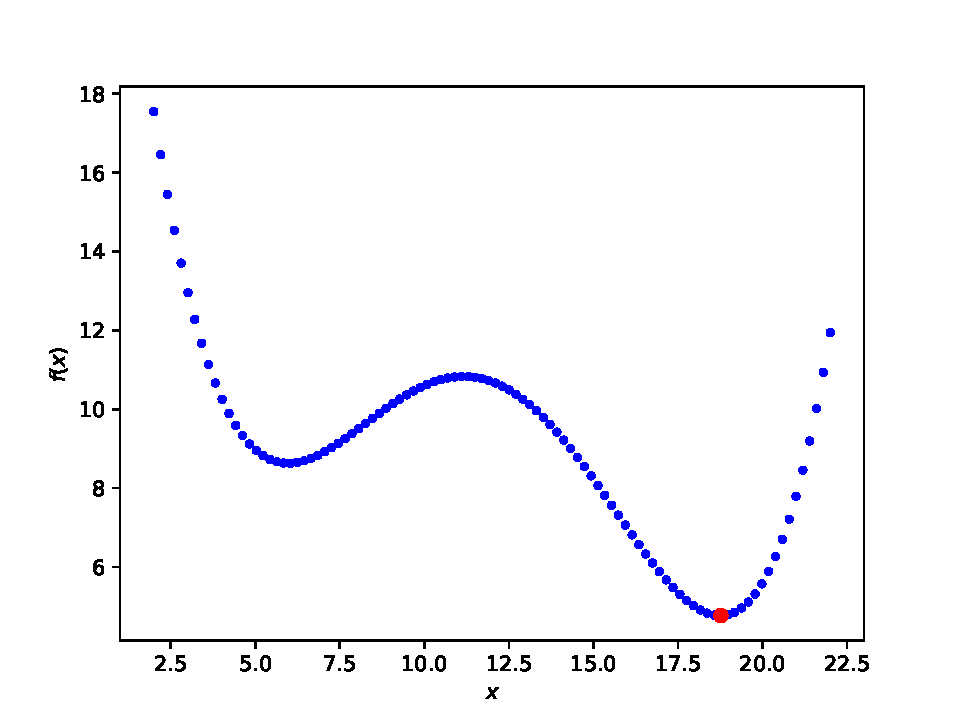
\includegraphics[width=0.8\textwidth]{./5_images/fig_grid_search_scalar.pdf} 
		\caption{Pesquisa em grade com número escalar}
		\label{fig:grid_search_scalar}
		\makebox[\width]{Fonte: Autor}
	\end{center}
\end{figure}

Ainda neste método, casos onde há uma maior quantidade de $x$ ($x_1$, $x_2$, \dots)
deve-se utilizar laços aninhados para que a varredura de todas as possibilidades
possa ser feita. 

Como exemplo, minimizemos a \cref{eq:grid_search_vect_no_bounds}, sendo
$0 \leq x_1 \leq 2$ e $1 \leq x_2 \leq 3$.

\begin{equation}
	\label{eq:grid_search_vect_no_bounds}
	f(x) = (x_1 - 1)^2 + (x_2 - 2)^2 + 0,5
\end{equation}

Neste caso, sem muito esforço notamos que
$f_{min} = 0,5$, $x_{1_{opt}} = 1$ e $x_{2_{opt}} = 2$.\footnote{
	O código-fonte em Python para este cálculo pode ser encontrado no
	\cref{ch:codigos_extras}, código \ref{lst:grid_search_vectorial}.}
Porém se a restrição da \cref{eq:grid_search_vect_bounds} for aplicada
encontramos os valores descritos nas equações descritas na \cref{eq:grid_search_vect_bounds_output}.

\begin{equation}
	\label{eq:grid_search_vect_bounds}
	f(x) = x_1 - x_2 + 1,5 \leq 0
\end{equation}

% \begin{subequations}
% 	\label{equ_grid_search_vect_bounds_output}
% 	\begin{align}
% 		f_{min} = 0,628 \\
% 		x_{1_{opt}} = 0,748 \\
% 		x_{2_{opt}} = 2,25
% 	\end{align}
% \end{subequations}

\begin{equation}
	\label{eq:grid_search_vect_bounds_output}
	\begin{aligned}
		f_{min} = 0,628 \\
		x_{1_{opt}} = 0,748 \\
		x_{2_{opt}} = 2,25
	\end{aligned}
\end{equation}

As figuras \ref{fig:grid_search_vectorial_nobounds} e \ref{fig:grid_search_vectorial_withbounds}
mostram a função custo (outra forma de chamarmos a função objetivo) sem restrição e com a
restrição descrita pela \cref{eq:min_restr_desigualdade}, respectivamente.

\begin{figure}[h]
    \centering
    \begin{minipage}{0.45\textwidth}
        \centering
        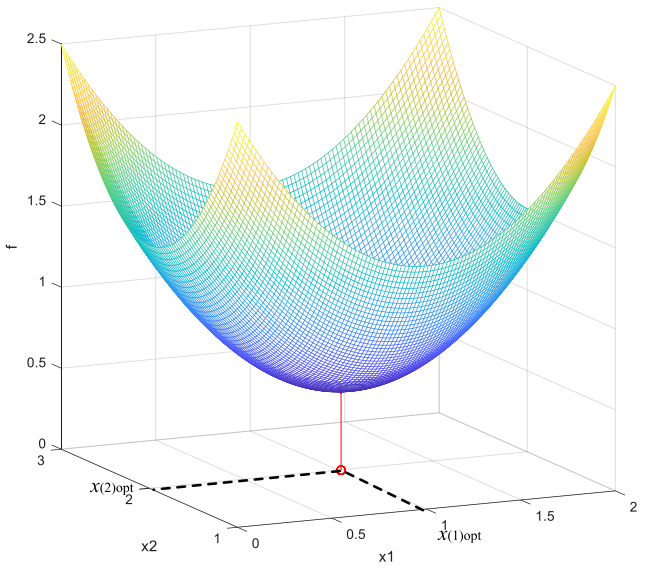
\includegraphics[width=0.9\textwidth]{./5_images/fig_grid_search_vectorial1.png} 
		\caption{Pesquisa em grade com duas variáveis e sem restrição}
		\label{fig:grid_search_vectorial_nobounds}
		Fonte: \citeonline{Haugen2018}
    \end{minipage}\hfill
    \begin{minipage}{0.45\textwidth}
        \centering
        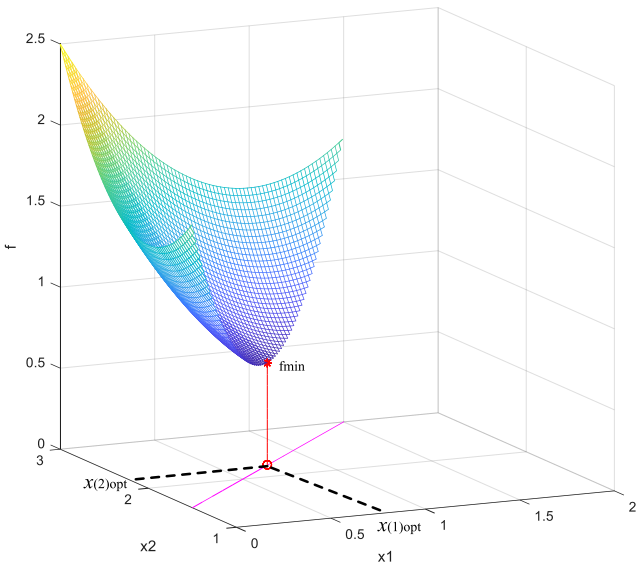
\includegraphics[width=0.9\textwidth]{./5_images/fig_grid_search_vectorial2.png} 
		\caption{Pesquisa em grade com duas variáveis e com restrição}  
		\label{fig:grid_search_vectorial_withbounds}		      
		Fonte: \citeonline{Haugen2018}
	\end{minipage}
\end{figure}

\subsection{Método de busca de descidas mais íngrimes}

Este método consiste em estimar o próximo valor de $x$ baseando-se na deriavada
da função custo calculada em $x$. Exemplificando para um caso escalar podemos dizer que
o próximo valor de $x$, isto é, $x_{k+1}$ será dado por:

\begin{align}
	\label{eq:steepest_decent_xk1}
	x_{k+1} &= x_k + \Delta x_k \\ 
	\Delta x_k &= -K f'(x_k)
\end{align}

\noindent
Onde: \\
$x_k$ = $x$ atual \\
$\Delta x_k$ = diferença entre $x_k$ e $x_{k+1}$ \\
$K$ = fator multiplicador do incremento \\
$f'(x_k)$ = derivada (ou gradiente) da função custo calculada em $x_k$ \newline

A derivada $f'(x_k)$ indica quão inclinada está a função custo no ponto $x_k$,
assim sendo o fator $K$ determina o peso que essa inclinação terá para o cálculo
do próximo valor de $x$.

A \cref{fig:steepest_decent_slope} mostra graficamente a influência da derivada
da função custo na amplitude de $\Delta x_k$ entre iterações.

\begin{figure}
	\begin{center}
		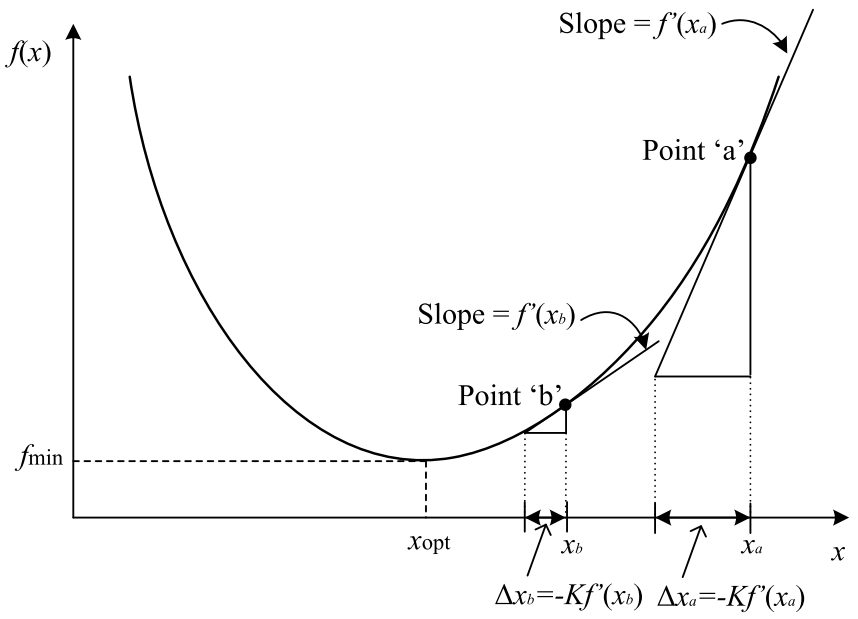
\includegraphics[width=0.75\textwidth]{./5_images/fig_steepest_decent_slope.png} 
		\caption{Influência de $f'(x_k)$ no cálculo de $x_{k+1}$ no método de descidas mais íngrimes}
		\label{fig:steepest_decent_slope}
		\makebox[\width]{Fonte: \citeonline{Haugen2018}}
	\end{center}
\end{figure}


\subsection{Método de Newton}

método de newton

\subsection{Otimizadores de programação não-linear (NLP)}

NLP

\section{Algumas aplicações de otimização}

\subsection{Estimação de parâmetros}

estimação de param

\subsection{Moving Horizon Estimation}

MHE

\subsection{Model Predictive Control}

MPC

\chapter{Controle Preditivo}
\label{ch:controle_preditivo}

% =====================================================================================================
% ============================================= Section ===============================================
% =====================================================================================================
\section{Introdução}

% TODO: Alguma intro

% =====================================================================================================
% ============================================= Section ===============================================
% =====================================================================================================
\section{Cronologia}
\label{sec:cronologia}

% TODO: Cronologia

% =====================================================================================================
% ============================================= Section ===============================================
% =====================================================================================================
\section{Elementos do controle preditivo}
\label{sec:elementos_do_controle_preditivo}

% TODO: Apresentacão

% .....................................................................................................
% ............................................ Subsection .............................................
% .....................................................................................................
\subsection{Modelo do processo}
\label{subsec:modelo_do_processo}

% TODO: Modleo 

% .....................................................................................................
% ............................................ Subsection .............................................
% .....................................................................................................
\subsection{Função Objetivo}
\label{subsec:funcao_objetivo}

% TODO: fun obj

% .....................................................................................................
% ............................................ Subsection .............................................
% .....................................................................................................
\subsection{Lei de Controle}
\label{subsec:lei_de_controle}

% TODO: lei de controle

% =====================================================================================================
% ============================================= Section ===============================================
% =====================================================================================================
\section{As diferentes estratégias do controle preditivo}
\label{sec:diferentes_estrategias_controle_preditivo}

% TODO: estrategias

% =====================================================================================================
% ============================================= Section ===============================================
% =====================================================================================================
\section{Estabilidade}
\label{sec:estabilidade}

% TODO: estabilidade

% .....................................................................................................
% ............................................ Subsection .............................................
% .....................................................................................................
\subsection{Controle Preditivo com Horizonte de Predição Infinito}
\label{subsec:controle_preditivo_com_horizonte_preditivo_infinito}

% TODO: Controle de predicao infiinito

% .....................................................................................................
% ............................................ Subsection .............................................
% .....................................................................................................
\subsection{Controle Preditivo Não-Linear}
\label{subsec:controle_preditivo_nao_linear}

% TODO: Não-linear

% =====================================================================================================
% ============================================= Section ===============================================
% =====================================================================================================
\section{Análise Complementar dos Sistemas de Controle}
\label{sec:analise_complementar_dos_sistemas_de_controle}

% TODO: analise complementar

% .....................................................................................................
% ............................................ Subsection .............................................
% .....................................................................................................
\subsection{Representação no Espaço de Estados}
\label{subsec:representacao_no_espaco_de_estados}

% TODO: Espaço de Estados

\chapter{Modelo Preditivo de Controle}
\label{cap_mpc}

\section{Introdução}

intro

\section{Algoritmos}

algo

\subsection{LQG}

LQG

\subsection{IDCOM}

IDCOM

\subsection{DMC}

DMC

\subsection{QDMC}

QDMC

\subsection{IDCOM-M, HIECON, SMCA e SMOC}

IDCOM-M

\subsection{DMC-plus e RMPCT In}

DMC-plus

% PARTE MATERIAIS E METODOS
\part{Materiais e métodos}

\chapter{Planta de controle de temperatura}
\label{ch:planta_de_controle_de_temperatura}

% TODO: APMonitor Lab

% PARTE RESULTADOS E DISCUSSAO
\part{Resultados e discussão}

\chapter{Plano de Trabalho e Cronograma}
\label{ch:plano_de_trabalho_e_cronograma}

% TODO: alguma introdução

% =====================================================================================================
% ============================================= Section ===============================================
% =====================================================================================================
\section{Plano de Trabalho}
\label{sec:plano_de_trabalho}

% TODO: plano de trablhao

% =====================================================================================================
% ============================================= Section ===============================================
% =====================================================================================================
\section{Cronograma}
\label{sec:cronograma}

% TODO: Cronograma


% ELEMENTOS PÓS-TEXTUAIS
\postextual

% Referências bibliográficas
\bibliography{./3_posText/library}

% Glossário
% Consulte o manual da classe abntex2 para orientações sobre o glossário.
% % ----------------------------------------------------------
% Glossário
% ----------------------------------------------------------

% ---
% Define nome e preâmbulo do glossário
% ---
\phantompart
%\renewcommand{\glossaryname}{Glossário}  A opção babel do glossaries faz a tradução.
\renewcommand{\glossarypreamble}{Esta é a descrição do glossário. Experimente
visualizar outros estilos de glossários, como o \texttt{altlisthypergroup},
por exemplo.\\
\\}

% ---
% Traduções para o ambiente glossaries
% ---  
% A opção babel do glossaries faz a tradução.

%\providetranslation{Glossary}{Glossário}
%\providetranslation{Acronyms}{Siglas}
%\providetranslation{Notation (glossaries)}{Notação}
%\providetranslation{Description (glossaries)}{Descrição}
%\providetranslation{Symbol (glossaries)}{Símbolo}
%\providetranslation{Page List (glossaries)}{Lista de Páginas}
%\providetranslation{Symbols (glossaries)}{Símbolos}
%\providetranslation{Numbers (glossaries)}{Números} 
% ---

% ---
% Estilo de glossário
% ---
% \setglossarystyle{index}
% \setglossarystyle{altlisthypergroup}
 \setglossarystyle{tree}  % Já selecionado no arquivo .sty 


% ---
% Imprime o glossário
% ---
\cleardoublepage
\phantomsection
\addcontentsline{toc}{chapter}{\glossaryname}
\printglossaries % imprime todas as entradas

\imprimirglossario  % não imprime acronimos (siglas) e nem simbolos
% ---

% Apêndices
\begin{apendicesenv}

% Imprime uma página indicando o início dos apêndices
\partapendices

% =====================================================================================================
% ============================================= Chapter ===============================================
% =====================================================================================================
\chapter{Códigos-fonte}
\label{ch:codigos_extras}

\section{Método de pesquisa em grade}

\lstinputlisting[	
	caption={Pesquisa em grade com número escalar},
	captionpos=t,
	label={lst:grid_search_scalar},
	language=Python,
	style=Python_lang]
	{./4_Codes/grid_search_scalar.py}
	\begin{center}
		\makebox[\width]{Fonte: Autor, adaptado de \citeonline{Haugen2018}}
	\end{center}

\section{Método de pesquisa em grade com duas variáveis}

\lstinputlisting[	
	caption={Pesquisa em grade com duas variáveis},
	captionpos=t,
	label={lst:grid_search_vectorial},
	language=Python,
	style=Python_lang]
	{./4_Codes/grid_search_vectorial.py}
	\begin{center}
		\makebox[\width]{Fonte: Autor, adaptado de \citeonline{Haugen2018}}
	\end{center}

\section{Exemplo do método \acrlong{mhe}}

% (Brincalepe): O código da página 44 deve ser deslocado para o apêndice.
% (cont.) Se quiser, destaque apenas alguma parte mais relevante e mantenha no corpo do texto.
\lstinputlisting[	
	caption={Exemplo do método \acrlong{mhe}},
	captionpos=t,
	label={lst:mhe_example},
	language=Python,
	style=Python_lang]
	{./4_Codes/mhe_example.py}
	\begin{center}
		\makebox[\width]{Fonte: Autor, adaptado de \citeonline{Haugen2018}}
	\end{center}

\section{Exemplo de aplicação do \acrlong{mpc}}

\lstinputlisting[	
	caption={Exemplo de aplicação do \acrlong{mpc}},
	captionpos=t,
	label={lst:mpc_example},
	language=Python,
	style=Python_lang]
	{./4_Codes/mpc_example.py}
	\begin{center}
		\makebox[\width]{Fonte: Autor, adaptado de \citeonline{Haugen2018}}
	\end{center}
% (Brincalepe): O código da página 58 também pode ser deslocado para o Apêndice.
% (cont.) Seria interessante descrevê-lo no corpo de texto através de um diagrama.

% =====================================================================================================
% ============================================= Chapter ===============================================
% =====================================================================================================
\chapter{Escolha da frequência de amostragem utilizando autocovariância}
\label{ch:sampling_time_using_autocorrelation}

A regra prática para a escolha da frequência de amostragem de sinal descrita por \citeonline{Aguirre2015}
e citada na \cref{subsubsec:periodo_de_amostragem} pode nem sempre ajudar muito, uma vez que é possível
que não se tenha nenhum conhecimento prévio do sinal para poder aplicar a regra de escolher uma frequência
de 5 a 10 vezes maior que a frequência de interesse \cite{Aguirre2015}. Para casos assim, \citeonline{Aguirre2015}
descreve uma outra técnica, que será apresentada nos parágrafos a seguir. 

Assume-se que o sinal já amostrado, $y^*(k)$, tenha sido obtido utilizando-se um tempo
de amostragem muito pequeno, ou seja, o sinal está superamostrado. Sendo assim, deseja-se encontrar o
valor $\Delta$ que descreva a fração pela qual o $y^*(k)$ pode ser decimado a fim de obter um sinal de trabalho
$y(k) = y^*(\Delta k)$, ou seja, o sinal decimado que ainda mantem as características originais do sinal $y^*(k)$.

Para fazer isso é necessário verificar o nível de correlação entre observações adjacentes do sinal
$y^*(k)$. Quanto mais superamostrado estiver o sinal $y^*(k)$, maior será a redundância entre duas
observações consecutivas. Este nível de correlação pode ser obtido calculando as funções de
autocovariância linear e não-linear (mostradas na \cref{eq:autocorrelation}) do sinal original.

\begin{subequations}
    \label{eq:autocorrelation}
    \begin{align}
		r_{y^*}(\tau) &= \mathrm{E} \left[(y^*(k) - \overline{y^*(k)}) (y^*(k - \tau) - \overline{y^*(k)})\right]		\\
		r_{y^{*2'}}(\tau) &= \mathrm{E} \left[(y^{*2}(k) - \overline{y^{*2}(k)}) (y^{*2}(k - \tau) - \overline{y^{*2}(k)})\right]
    \end{align}
\end{subequations}

$\mathrm{E}[\cdot]$ indica a esperança matemática, porém, sendo $y^*(k)$ ergótico, $\mathrm{E}[\cdot]$
pode ser substituída pela média temporal.

Após calculados $r_{y^*}(\tau)$ e $r_{y^{*2'}}(\tau)$, determinam-se seus primeiros mínimos,
$\tau_{y^*}$ e $\tau_{y^{*2'}}$, respectivamente. O menor desses mínimos passa a ser o valor de trabalho
$\tau_{m}^{*}$, ou seja, $\tau_{m}^{*} = \mathrm{min} \left[ \tau_{y^*} , \tau_{y^{*2'}} \right]$.

Por fim, deseja-se escolha $\Delta$ de forma que as funções de autocovariância do sinal decimado $y(k) = y^*(k)$
satisfaçam

\begin{equation}
    \label{eq:tau_m}
    10 \leq \tau_m \leq 20
\end{equation}

\noindent
sendo que $\tau_m$ é definido pelo sinal decimado $y(k)$ de maneira análoga a $\tau_m^*$ para o
sinal $y^*(k)$. Os limites inferior e superior da \cref{eq:tau_m} podem ser relaxados para
$5$ e $10$, respectivamente.

% =====================================================================================================
% ============================================= Section ===============================================
% =====================================================================================================
\section{Aplicação prática}
\label{ch:using_sampling_time_with_autocorrelation}

As \cref{fig:rise_time_sensor1,fig:rise_time_sensor2} da \cref{subsubsec:periodo_de_amostragem}
apresentam a resposta dos sensores de temperatura do \acrshort{tclabsp} quando o Aquecedor 1 é
excitado com um degrau de 0 à 50\%.

Após alguns testes preliminares, foi observado que o sistema apresentava uma resposta lenta
e que, portanto, uma coleta de dados com tempo de amostragem de $0.25s$ seria suficiente para
superamostrar os dados e garantir que todas as características de resposta do sistema tenham
sido amostradas.

Calcula-se então as funções de autocovariância apresentadas na \cref{eq:autocorrelation} para os
sensores de temperatura 1 e 2, como apresentado na \cref{fig:autocorrelationS1S2}.

\begin{figure}[h]
	\caption{Funções de autocovariância dos Sensores de Temperatura 1 e 2}
	\begin{center}
		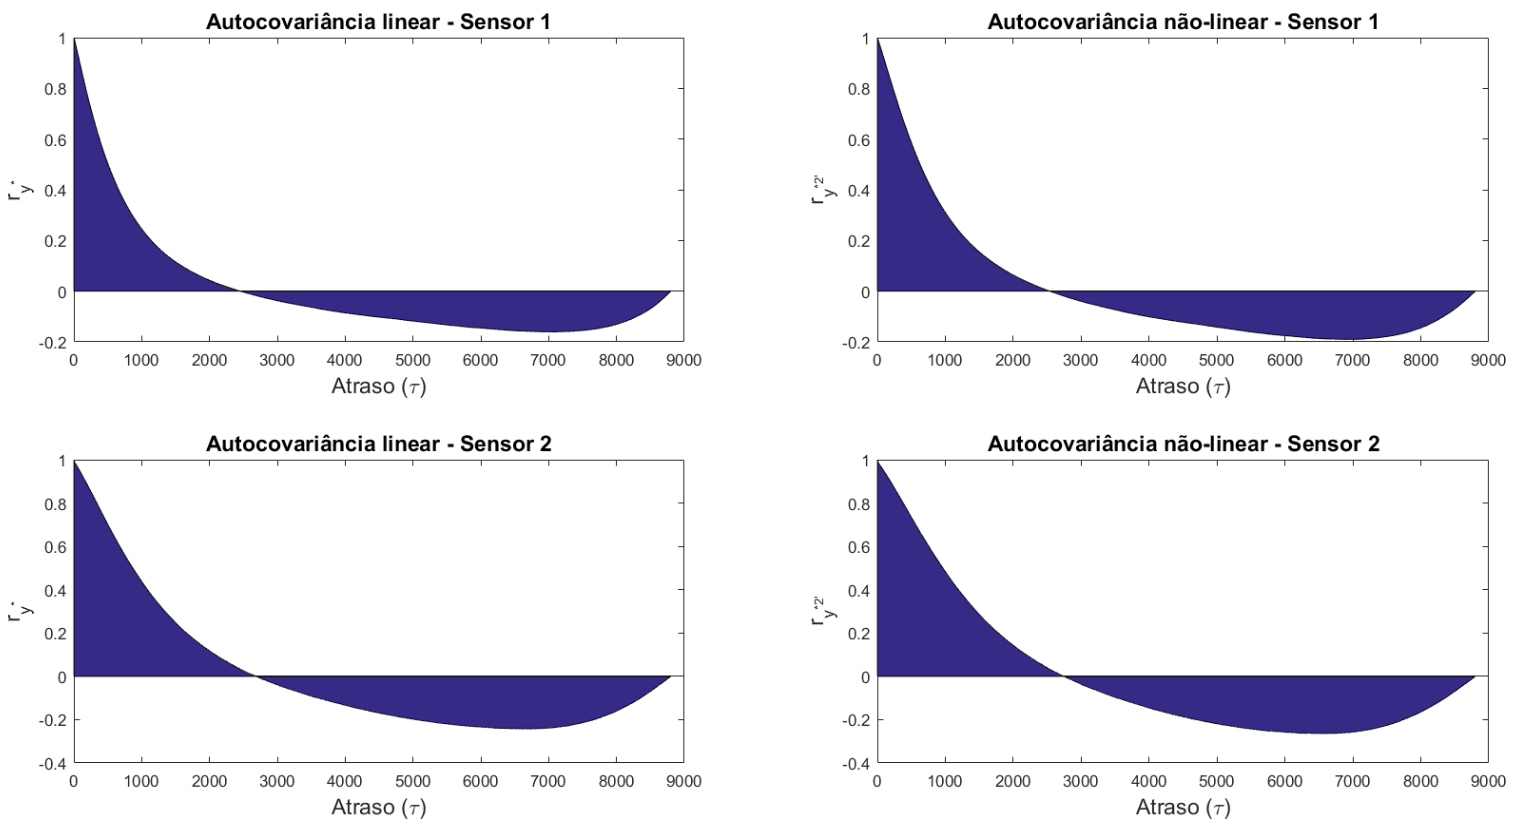
\includegraphics[width=0.95\textwidth]{./5_images/AutocorrelationS1S2.png} 
		\label{fig:autocorrelationS1S2}
	\end{center}
	\centering
	\makebox[\width]{Fonte: \citeonline{Prata2019}} 
\end{figure}

Para cada um dos sensores, encontramos então o valor mínimo das funções de autocovariância
($\tau_{y^{*}}$ e $\tau_{y^{*2'}}$), e a partir delas determinamos $\tau_m^*$
($\tau_{m}^{*} = \mathrm{min} \left[ \tau_{y^*} , \tau_{y^{*2'}} \right]$).
O resultado é apresentado na \cref{tab:tau_s1s2}.

\begin{table}[h]
	\centering
	\caption{Mínimos das funções de autocovariância}
	\label{tab:tau_s1s2}
	\begin{tabular}{llll} \toprule
		{Sensor}		& {$\tau_{y^{*}}$}		& {$\tau_{y^{*2'}}$}		& {$\pmb{\tau}_{\pmb{m}}^{\pmb{*}}$}		\\ \midrule
		Sensor 1		& $7015$				& $6925$					& $\pmb{6}\pmb{9}\pmb{2}\pmb{5}$			\\
		Sensor 2		& $6735$				& $6621$					& $\pmb{6}\pmb{6}\pmb{2}\pmb{1}$			\\ \bottomrule
	\end{tabular}
	\caption*{Fonte: Autor}
\end{table}

Conhecendo $\tau_{m}^{*}$ é possível encontrar um valor de $\Delta$ para obter o sinal decimado
$y(k) = y^*(\Delta k)$, tal que o valor mínimo da suas funções de autocovariância satisfaçam
\cref{eq:tau_m}.

Uma demonstração do efeito da variação do $\Delta$ no tempo de amostragem do sinal
pode ver vista na \cref{tab:delta_action}

\begin{table}[h]
	\centering
	\caption{Efeito do $\Delta$ no tempo de amostragem}
	\label{tab:delta_action}
	\begin{tabular}{cccccc} \toprule
		{k}		& {$\Delta=1$}		& {$\Delta=2$}		& {$\cdots$}	& {$\Delta=4$}	& {$\cdots$} 	\\ \midrule
		1		& $0.00$			& $0.00$			& \hfill		& $0.00$		& \hfill		\\
		2		& $0.25$			& $0.50$			& \hfill		& $1.00$		& \hfill		\\
		3		& $0.50$			& $1.00$			& \hfill		& $2.00$		& \hfill		\\
		4		& $0.75$			& $0.50$			& \hfill		& $3.00$		& \hfill		\\
		5		& $1.00$			& $2.00$			& \hfill		& $4.00$		& \hfill		\\ \bottomrule 
	\end{tabular}
	\caption*{Fonte: Autor}
\end{table}

Através de um algoritmo\footnote{
	Indicar algoritmo utilizado			% TODO Indicar algoritmo utilizado
} foi possível testar diferentes valores de $\Delta$ a fim de encontrar
aquele que primeiro satisfizesse a \cref{eq:tau_m}, e por meio deste algoritmo encontrou-se
os valores de $\Delta$ e de $T_s$ (tempo de amostragem) indicados da \cref{eq:delta_and_ts}.

\begin{subequations}
    \label{eq:delta_and_ts}
    \begin{align}
		\Delta &= 253	\\
		T_s &= 63.25s
    \end{align}
\end{subequations}


\end{apendicesenv}


% Anexos
%\begin{anexosenv}

% Imprime uma página indicando o início dos anexos
\partanexos

\chapter{fmincon}
\label{ch:fmincon}

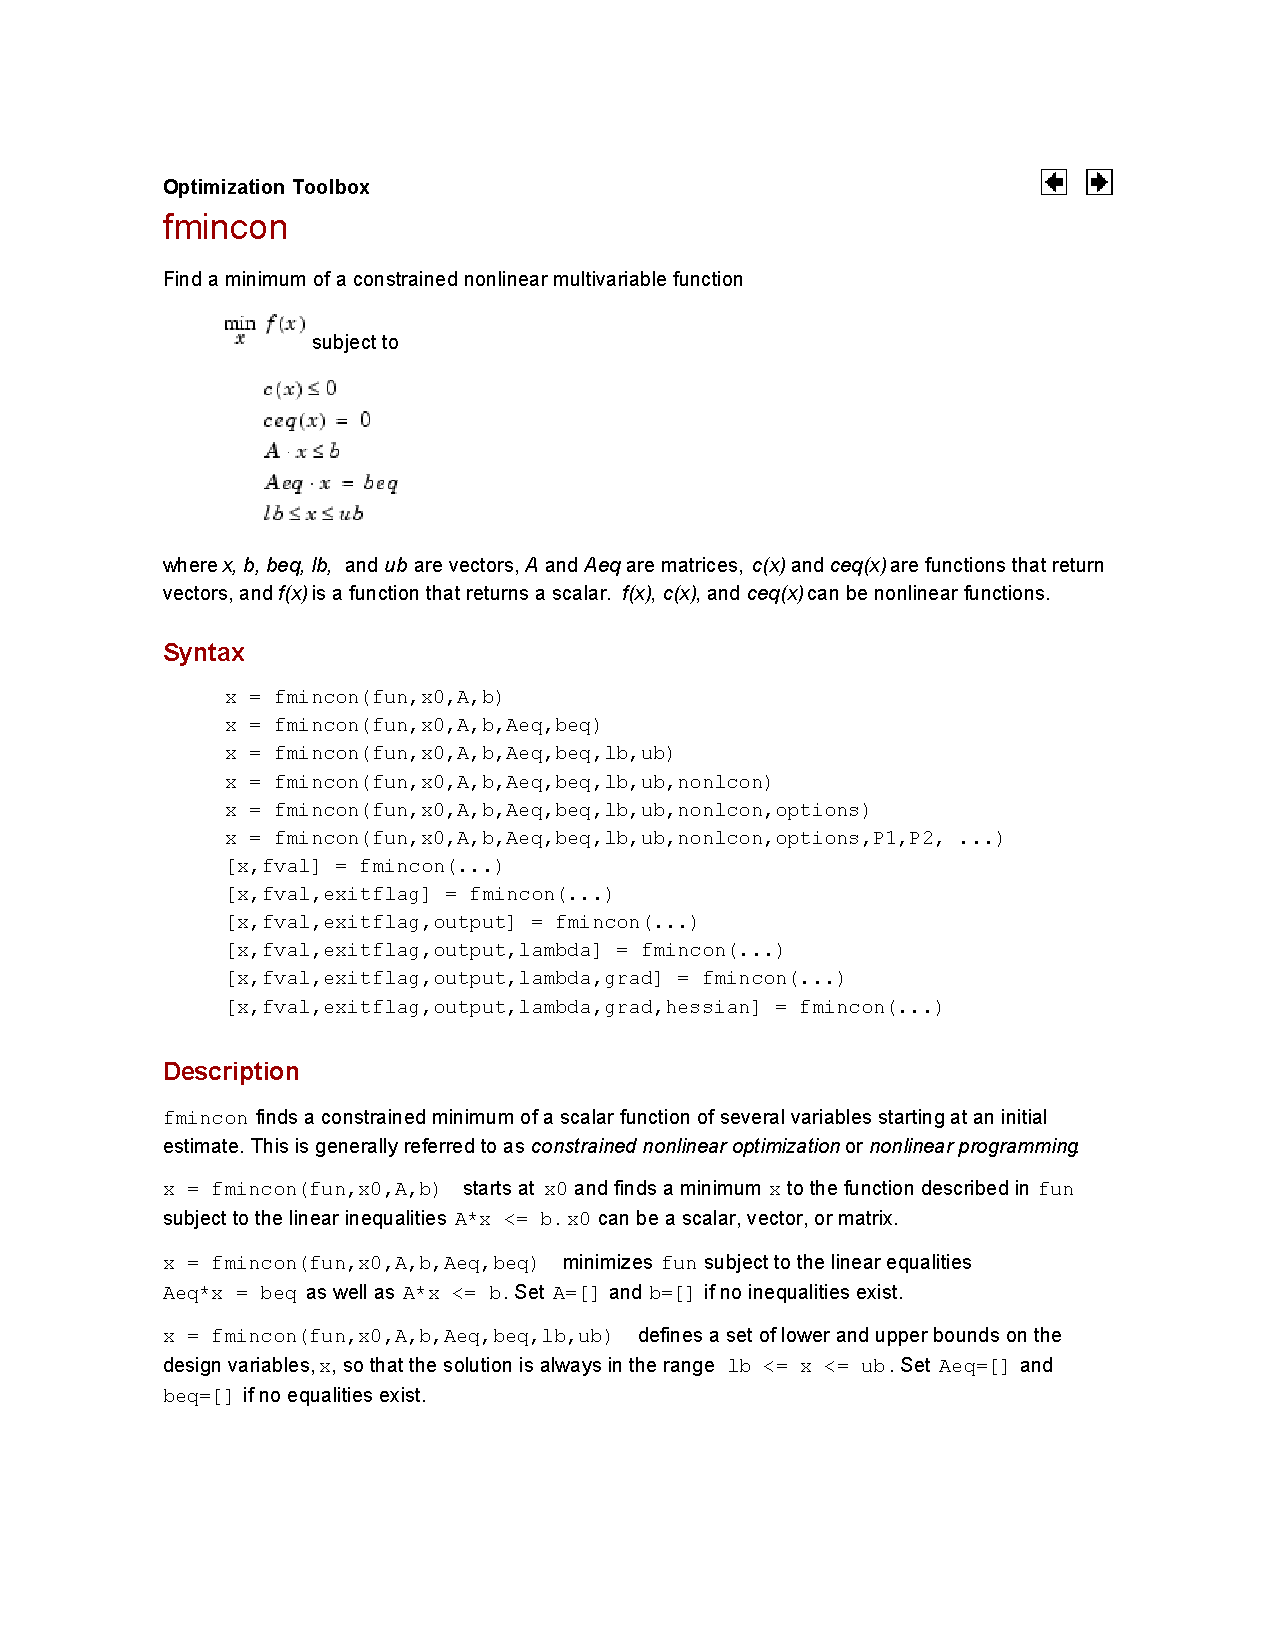
\includepdf[pages=-]{6_annex/fmincon.pdf}

\chapter{scipy.optimize.minimize}
\label{ch:scipy_optimize_minimize}

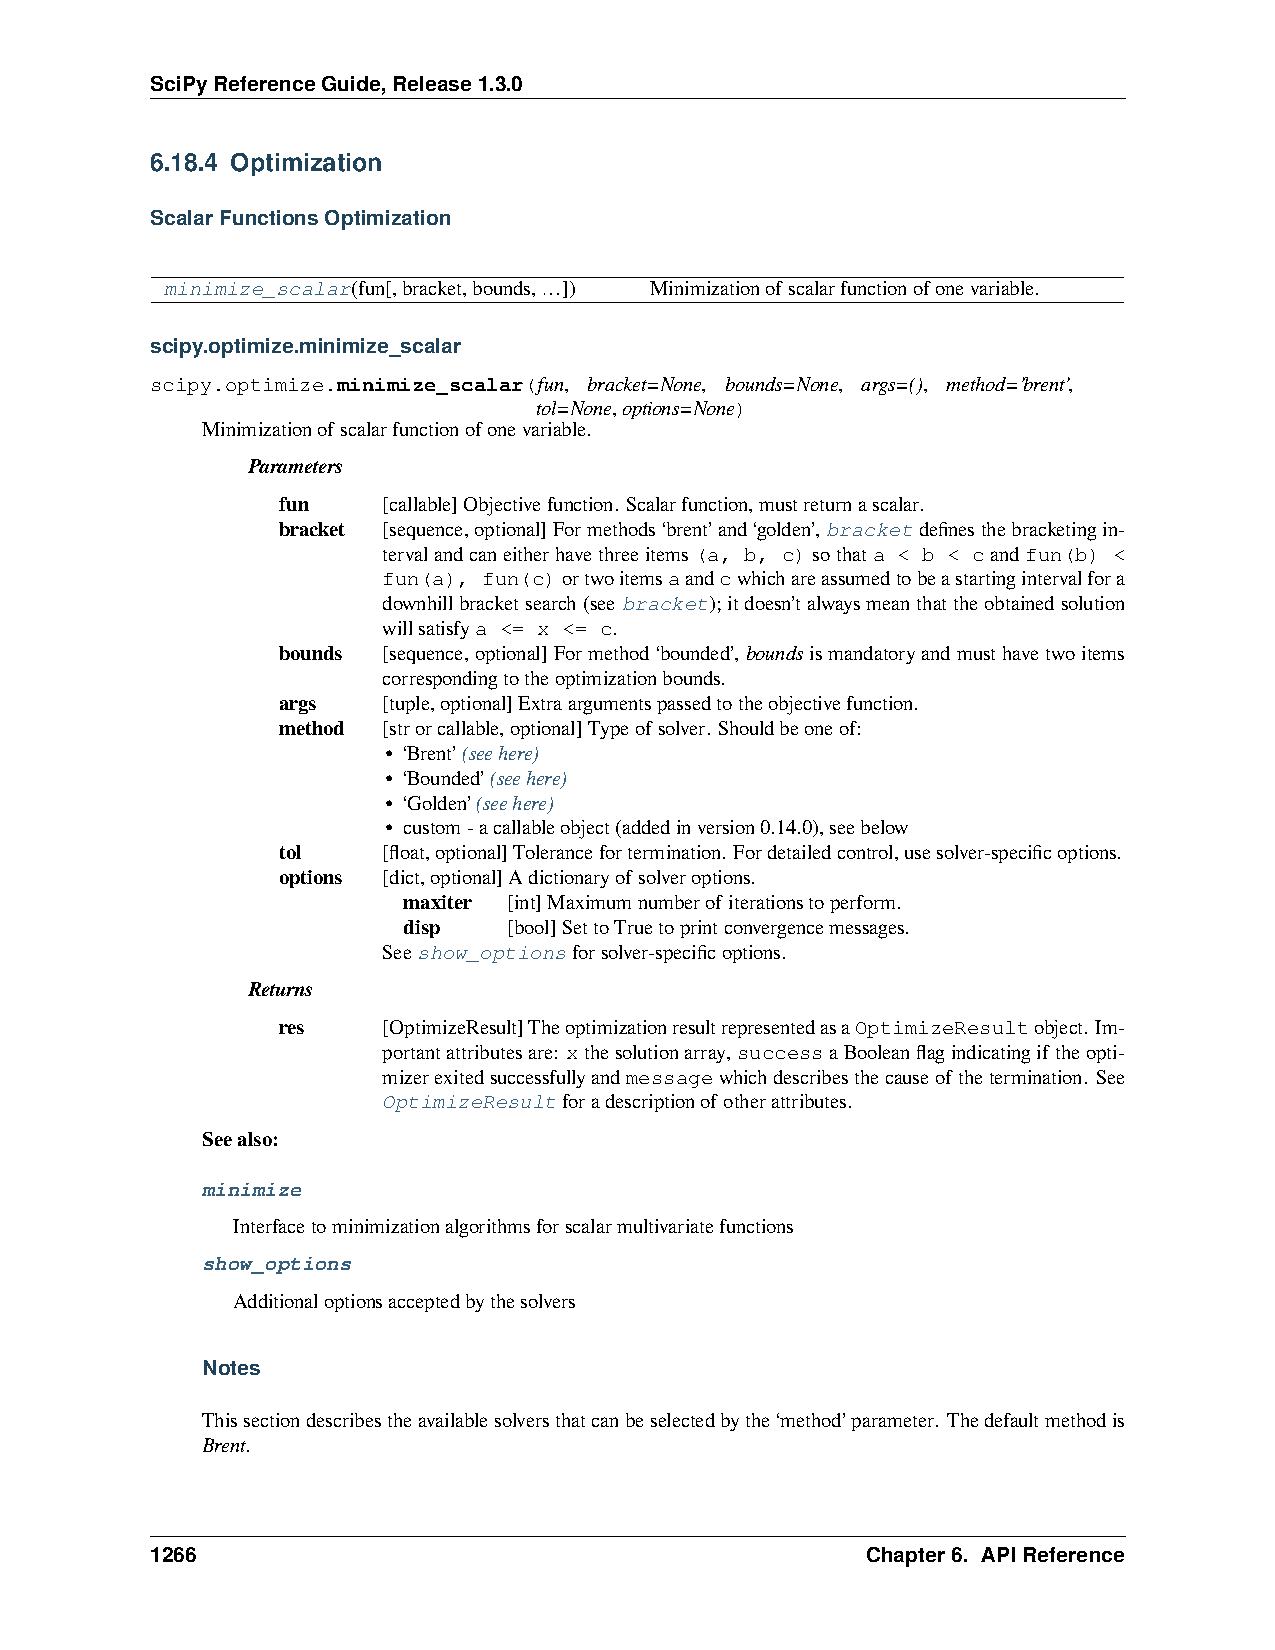
\includepdf[pages=-]{6_annex/scipy_optimize_minimize.pdf}


\end{anexosenv}


% INDICE REMISSIVO
\phantompart
\printindex

\end{document}
